\documentclass[a4paper,12pt]{article}
\usepackage[a4paper,top=1.3cm,bottom=2cm,left=1.5cm,right=1.5cm,marginparwidth=0.75cm]{geometry}
\usepackage{setspace}
\usepackage{cmap}
\usepackage{mathtext}
\usepackage[T2A]{fontenc}
\usepackage[utf8]{inputenc}
\usepackage[english,russian]{babel}
\usepackage{multirow}
\usepackage{graphicx}
\usepackage{wrapfig}
\usepackage{tabularx}
\usepackage{bm}
\usepackage{float}
\usepackage{longtable}
% \usepackage{upgreek}
\usepackage{hyperref}
\usepackage{textcomp}
\hypersetup{pdfstartview=FitH,  linkcolor=linkcolor,urlcolor=urlcolor, colorlinks=true}
\hypersetup{
    colorlinks=true,
    linkcolor=blue,
    filecolor=magenta,
    urlcolor=cyan,
    pdftitle={Overleaf Example},
    pdfpagemode=FullScreen,
    }
\usepackage[rgb]{xcolor}
\usepackage{amsmath,amsfonts,amssymb,amsthm,mathtools}
\usepackage{icomma}
\mathtoolsset{showonlyrefs=true}
\usepackage{euscript}
\usepackage{mathrsfs}
\usepackage{ dsfont }
\linespread{1.25}
\date{}
\DeclareMathOperator{\rg}{rg}
\DeclareMathOperator{\im}{Im}
\DeclareMathOperator{\mker}{Ker}
\DeclareMathOperator{\tr}{tr}
\DeclareMathOperator{\det}{det}

\definecolor{my-cyan}{RGB}{0, 153, 153}
\definecolor{my-purple}{RGB}{148, 0, 211}
\definecolor{my-red}{RGB}{248, 23, 62}
\definecolor{my-orange}{RGB}{255, 153, 0}

\graphicspath{{images/}}

\begin{document}

\begin{titlepage}
	\begin{center}
		\large 	Московский физико-технический институт \\
		\vspace{0.2cm}

		\vspace{4.5cm}
		\LARGE \textbf{Вопрос по выбору} \\ \vspace{0.2cm}
		\large (Общая физика: электричество и магнетизм) \\ \vspace{0.2cm}
		\LARGE \textbf{ЭЛЕКТРОМАГНИТНЫЕ ВОЛНЫ В
ВОЛНОВОДАХ}
	\end{center}
	\vspace{2.3cm} \large

	\begin{center}
		Работу выполнили: \\
        Лазарь Владислав, группа Б01-202\\
        Загороднюк Владислав, группа Б01-202\\
	\end{center}
	\begin{center} \vspace{90mm}
		г. Долгопрудный \\
		 Декабрь, 2023 год
	\end{center}
\end{titlepage}

\section*{Цель работы}
Ознакомление с методами получения и анализа электромагнитных волн СВЧ-диапазона.

\section*{В работе используются}
Генератор СВЧ типа Г4-83, измерительная линия Р1-28, усилитель 28 ИМ, заглушка, отрезок волновода с поглощающей нагрузкой, отрезки волноводов различных сечений, детекторная головка.

\section*{Теоретические сведения}

\subsection*{1. Волны СВЧ и волноводы}
\begin{wrapfigure}{r}{0.3\textwidth}
  \begin{center}
    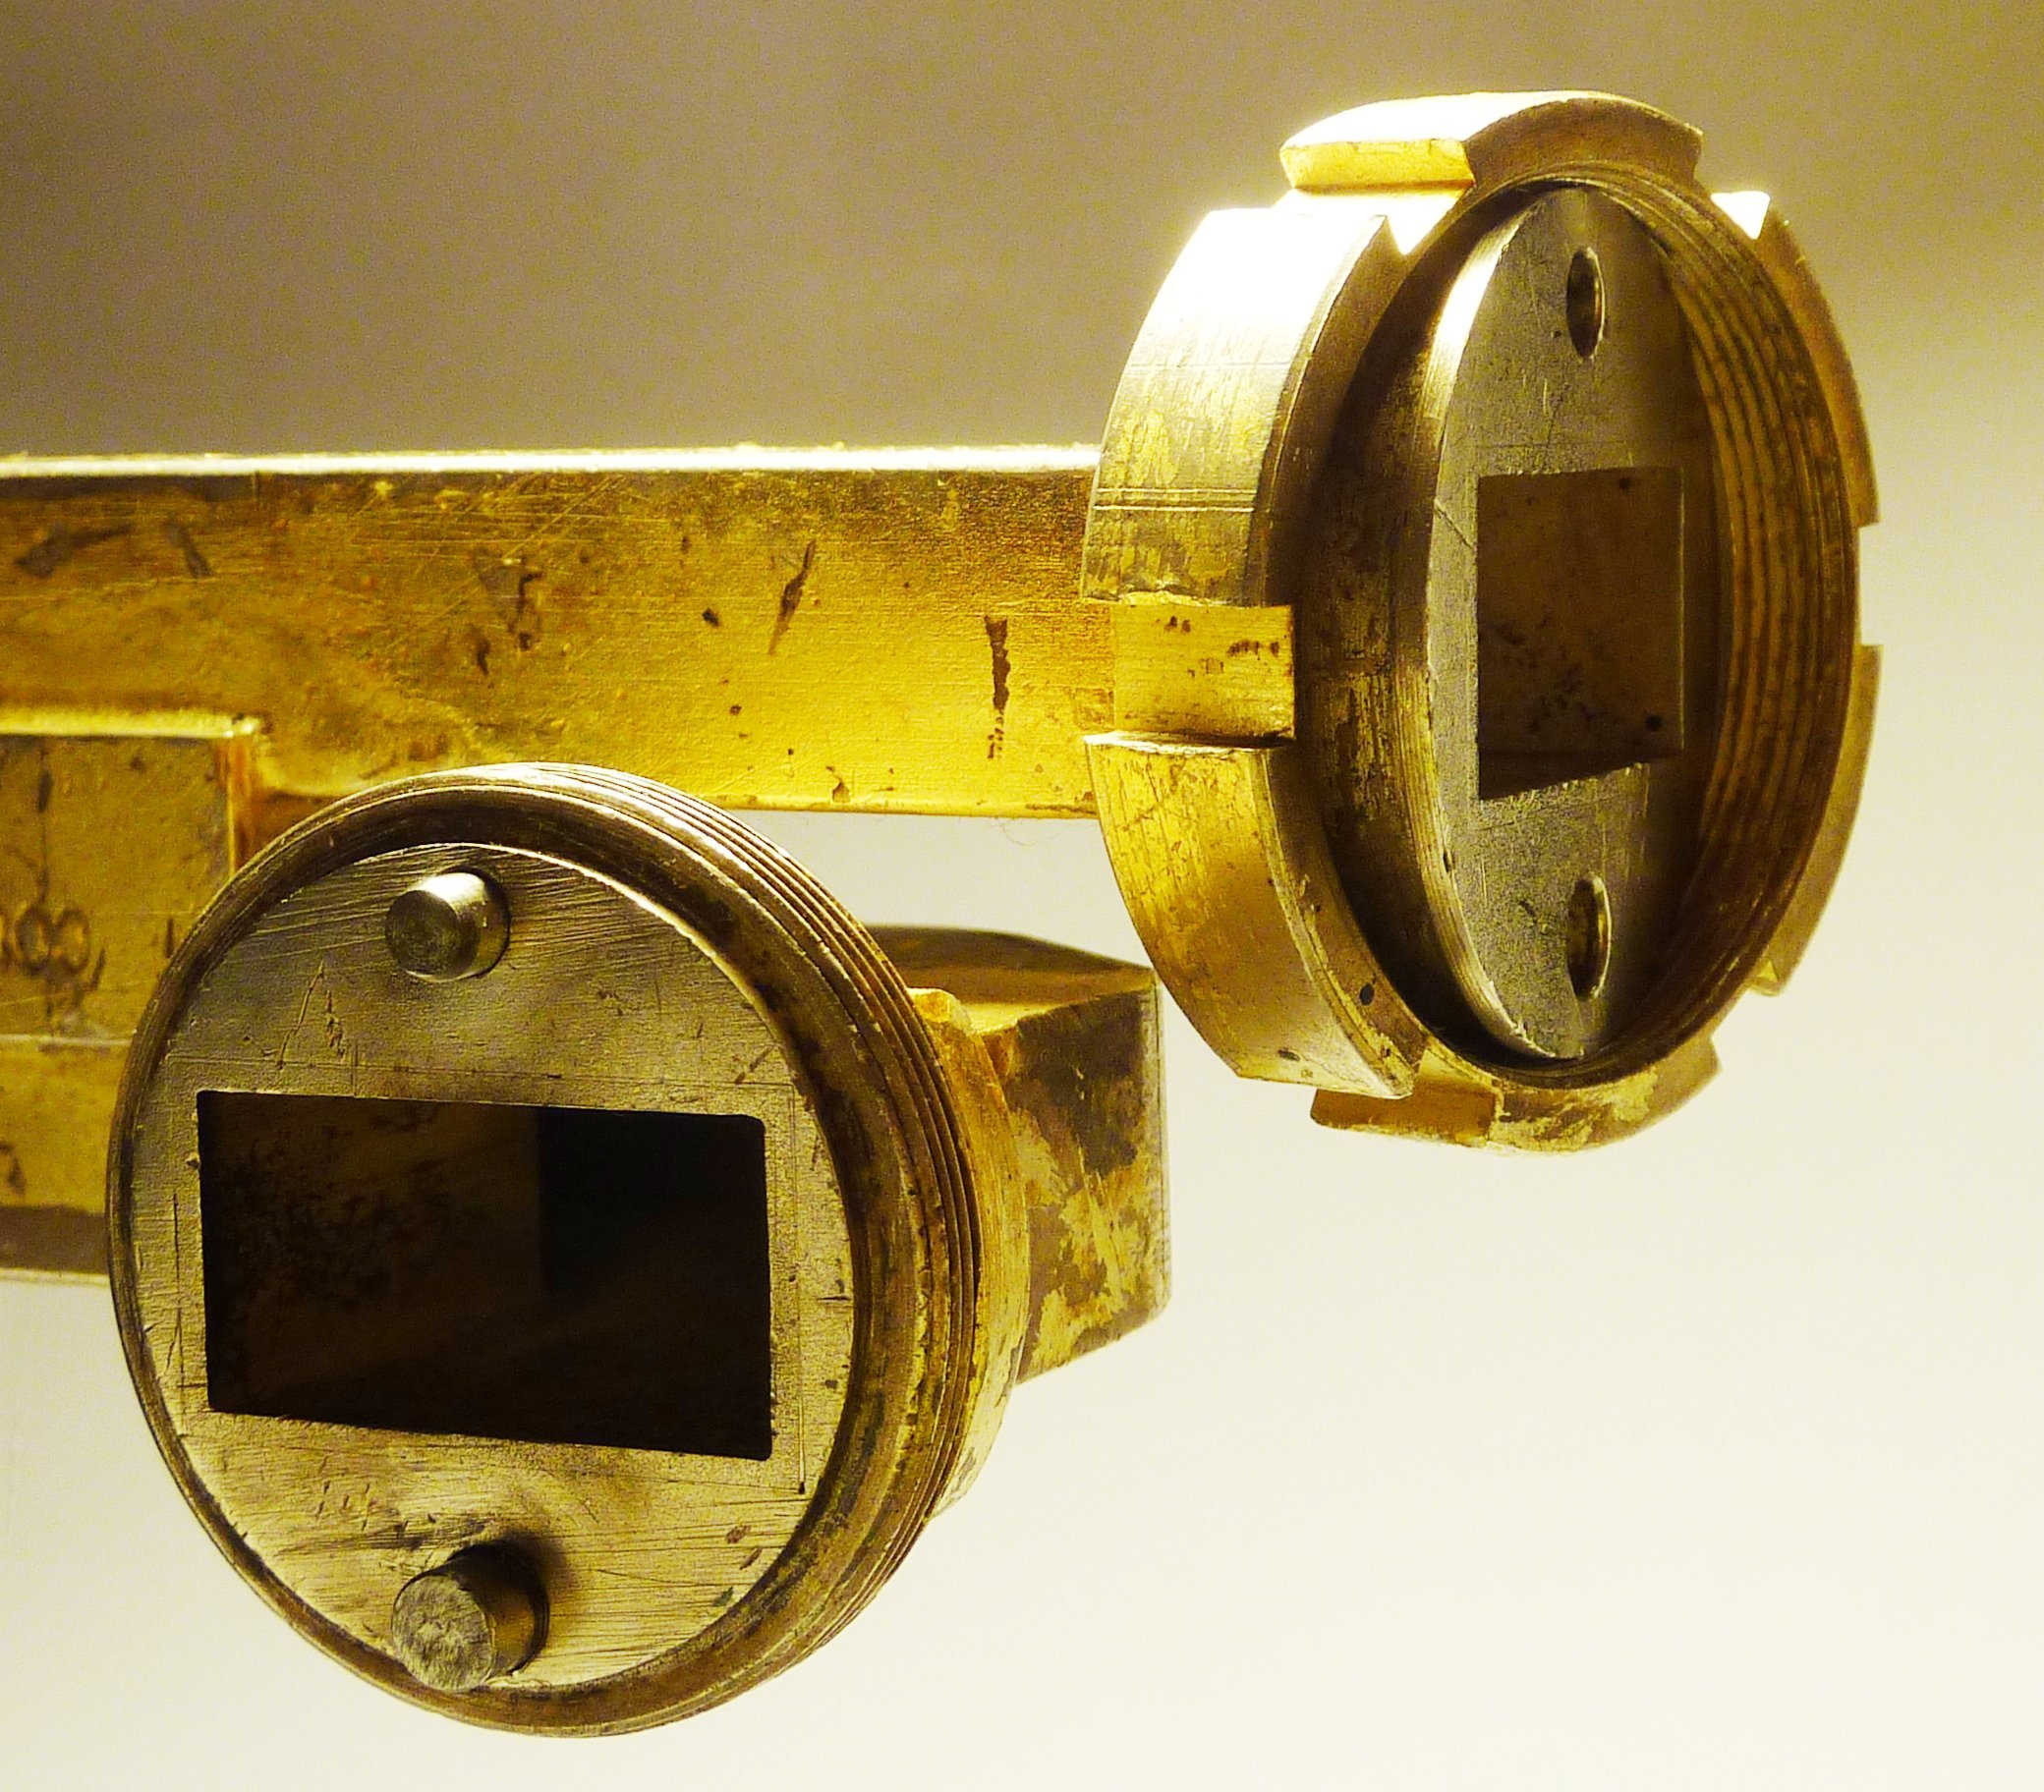
\includegraphics[width=0.29\textwidth]{images/waveguide.jpg}
  \end{center}
  \caption{Металлический волновод}
\end{wrapfigure}
Диапазон электромагнитных волн с частотой от 300 МГц до 300 Гц, или же с длиной волны от 1 метра до 1 миллиметра, называется диапазоном сверхвысоких частот, или же СВЧ. Передача электромагнитной энергии с помощью двухпроводной линии или коаксиальных кабелей становится малоэффективной из-за больших потерь: во-первых, резко возрастает сопротивление проводов из-за скин-эффекта, а в двухпроводной линии, кроме того, потери растут вследствие излучения энергии в окружающее пространство.
В СВЧ-диапазоне энергия передаётся с помощью волноводов - труб, сделанных из металла или диэлектрика (в миллиметровом диапазоне). Электромагнитные волны могут распространяться по металлическим трубам любого профиля, но из технологических соображений сечения волноводов делаются либо круглыми, либо прямоугольными.

\subsection*{2. Концепция Бриллюэна}

В концепции Бриллюэна мы рассматриваем э.м. поле в волноводе как сумму падающей и отражённой от стенок плоских волн.

\begin{wrapfigure}{r}{0.3\textwidth}
  \begin{center}
    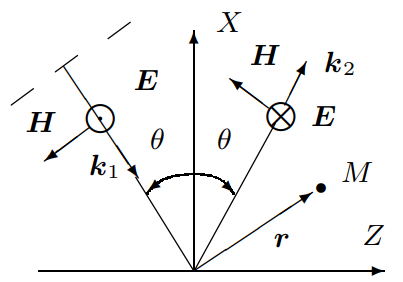
\includegraphics[width=0.29\textwidth]{images/reflection.jpg}
  \end{center}
  \caption{Отражение волны от поверхности металла}
\end{wrapfigure}

Рассмотрим отражение плоской э.м. волны от идеально проводящей,
бесконечно протяжённой плоской поверхности x = 0 (рис. 2). Пусть вектор напряжённости электрического поля падающей волны $E$ параллелен
этой плоскости. В наших обозначениях вектор $E_{пад}$ направлен по оси Y
(на нас). Фронт волны, падающей под углом $\theta$ к нормали, показан на
рис. 1 пунктиром. Оба вектора напряжённости $E$ и $H$ лежат в плоскости
фронта волны, им перпендикулярен волновой вектор $k$, описывающий
распространение волны.\\
Для модуля вектора $k$ (волнового числа) действительно выражение:
\begin{equation}
    k = \frac{2\pi}{\lambda} = \frac{\omega}{V_{\text{Ф}}}
\end{equation}
где $V_{\text{Ф}}$ - фазовая скорость волны, совпадающая со скоростью света в пустом пространстве.\\
Рассмотрим произвольную точку M - в неё приходят сразу две волны - падающая $E_{\text{пад}}$ и отражённая $E_{\text{отр}}$:
\begin{equation}
    E_{\text{пад}} = E_0 \cdot e^{i(\omega t - \mathbf{k_1 r})}, E_{\text{отр}} = - E_0 \cdot e^{i(\omega t - \mathbf{k_2 r})}
\end{equation}
По модулю $k_1 = k_2 = \frac{\omega}{c}$, тогда как их проекции на оси координат:
\begin{equation}
    k_{1x} = -k_{2x} = -k \cos \theta, k_{1z} = k_{2z} = k \sin \theta
\end{equation}
При отражении волны от проводящей поверхности происходит сдвиг фаз в $180^{\circ}$, откуда и появляется знак - в выражении электрической напряжённости отражённой волны.
Тогда имеем выражение для суммарного электрического поля в точке M:
\begin{equation}
    E = E_0 (e^{i(\omega t - \mathbf{k_1 r})} - e^{i(\omega t - \mathbf{k_2 r})})
\end{equation}
Или, подставляя компоненты вектора $\mathbf{r} = (x, 0, z)$, а также компоненты вектора $\mathbf{k}$, получаем:
\begin{equation}
    E = 2i E_0 \sin(k x \cos \theta) e^{i \omega (t - z \sin{\frac{\theta}{c}})}
\end{equation}
Мы получили уравнение волны в точке M с амплитудой $2 i E_0 \sin (k x \cos \theta)$ и фазовой скоростью $\frac{c}{\sin \theta}$.
Отметим две важные особенности этой волны: 1) её фазовая скорость
больше скорости света; 2) при фиксированном угле $\theta$ амплитуда поля
гармонически зависит от $x$ и не меняется со временем. Иначе говоря, в результате интерференции падающей и отражённой волн в пространстве над проводящей поверхностью в направлении оси X образуется система стоячих волн. Электрическое поле стоячей волны равно нулю в точках, где $k x \cos \theta = n \pi$, т.е. там, где
\begin{equation}
    x = \frac{n \pi}{k \cos \theta}
\end{equation}
Таким образом, поверхность нулевого электрического поля представляет собой плоскость, параллельную отражающей поверхности. Расположим в этой плоскости вторую проводящую поверхность. Эта поверхность не исказит полученного распределения поля, т.к. на ней автоматически удовлетворяются граничные условия $E(t) = 0$. Точно такие же плоскости
можно поставить, например, при $y = 0$ и $y = b$. Эти плоскости нормальны электрическим силовым линиям, и на них выполняются граничные
условия.
Итак, мы показали, что в волноводе прямоугольного сечения может распространяться э.м. волна, которую в пределах волновода можно рассматривать как результат суперпозиции двух плоских волн. Каждая плоская волна является чисто поперечной, так что электрическое и магнитное поля перпендикулярны к направлению их распространения.
В суммарной волне электрическое поле имеет только составляющую $E_y$ и, следовательно, перпендикулярно оси волновода, а магнитное поле имеет составляющие $H_x$ и $H_z$. Электромагнитное поле в волноводе не является чисто поперечным, а имеет продольные составляющие. В рассмотренном случае отлична от нуля продольная составляющая магнитного поля, и поэтому такую волну называют магнитной (H-волна). Мы могли бы взять другую поляризацию исходной падающей волны ($H = H_y$), и тогда возникла бы электрическая волна с $E_z \neq 0$ (E-волна). Посмотрим на вышеприведённое соотношение с другой стороны. Если даны две параллельные проводящие плоскости, расположенные на расстоянии $a$ друг от друга, то между ними могут распространяться волны, если
\begin{equation}
    \cos \theta_n = \frac{n \pi}{k a} = \frac{n \lambda_0}{2 a} = \frac{n \pi c}{a \omega}
\end{equation}
где $\lambda_0$ - длина волны в свободном пространстве. То есть движение э.м. волны по волноводу возможно только при выполнении условия:
\begin{equation}
    \cos \theta_n = \frac{n \lambda_0}{2 a} \leq 1
\end{equation}
поэтому для каждого n существует наибольшая критическая длина волны и соответственно наименьшая критическая частота, при которых волна ещё может проходить через волновод. Они равно, соответственно, $\omega_{\text{кр}} = \frac{\pi c}{a}$ и $\lambda_{\text{кр}} = 2a$.\\
Тогда мы можем найти выражение для фазовой скорости э.м. волны:
\begin{equation}
    v_{\text{Ф}} = \frac{c}{\sin \theta} = \frac{c}{\sqrt{1-\cos^2 \theta}} = \frac{c}{\sqrt{1 - \left(\frac{\omega_{\text{кр}}}{\omega}\right)^2}}
\end{equation}
Фазовая скорость (скорость перемещения поверхности постоянной фазы $v_{\text{Ф}} = \frac{\omega}{k}$) в волноводе больше скорости света в пустоте, а групповая скорость (скорость распространения возмущения $u = \frac{d\omega}{dk}$) всегда меньше. Интересно отметить, что фазовая скорость зависит от частоты. В таких случаях говорят, что среда (в данном случае — волновод) обладает дисперсией.
Подставив полученное выражение в самое первое уравнение нашей теорсправки, можно найти волновое число $k_z$, описывающее распространение волны вдоль волновода:
\begin{equation}
    k_z = \frac{\omega}{v_{\text{Ф}}} = \frac{\omega}{c} \sqrt{1 - \frac{\omega_{\text{кр}}}{\omega}}
\end{equation}
Из этого выражения следует, что по мере убывания частоты волновое число
$k_z$ уменьшается и, наконец, при $\omega < \omega_{\text{кр}}$ (или, что тоже, $\lambda_0 > 2a$)
оно становится мнимым. Это означает, что при частотах $\omega < \omega_{\text{кр}} = \frac{\pi c}{a}$ волны вдоль трубы экспоненциально затухают. Поэтому критическую частоту называют граничной частотой волновода.
Преобразуя это соотношение, можно связать длины волн в волноводе ($\lambda_{\text{В}}$), в открытом пространстве ($\lambda_0$) и критическую ($\lambda_{\text{кр}}$):
\begin{equation}
    \frac{1}{\lambda^2_B} = \frac{1}{\lambda^2} - \frac{1}{\lambda_{\text{кр}}}
\end{equation}
Ясно, что никакой выделенности оси X нет, и поэтому точно так же может образоваться синусоидальное распределение поля и вдоль оси Y. Поэтому для каждого вида E- и H-волны получается бесчисленное множество решений, каждое из которых имеет свою критическую частоту и длину волны. В случае прямоугольного волновода с поперечными размерами $a$ и $b$ все возможные критические длины волн определяются общей формулой:
\begin{equation}
    \lambda|{\text{кр}} = \frac{1}{\sqrt{(\frac{m}{2a})^2 + (\frac{n}{2b})^2}}
\end{equation}

где $m$ и $n$ — целые числа. Величина $m$ представляет собой полное число полупериодов изменения той или иной составляющей поля вдоль пути, идущего параллельно широкой стенке волновода (a), а $n$ — то же для узкой стенки (b). Эти же символы употребляются и в обозначениях волн — соответственно $E_{mn}$ или $H_{mn}$. . Обычно для передачи СВЧ-энергии по прямоугольным волноводам используется волна $H_{10}$. Её критическая длина волны — максимальная среди всех типов волн в прямоугольном волноводе, и поэтому её называют \textit{основной}. Тем самым, для волновода заданного сечения существует диапазон частот, ограниченный снизу критической частотой волны $H_{10}$ ($\lambda_{\text{кр}} = 2a$), а сверху — критической частотой следующей распространяющейся волны (например, $H_{10}$ с $\lambda_{\text{кр}} = 2b$ или $H_{20}$ с $\lambda_{\text{кр}} = a$). В этом частотном диапазоне СВЧ-энергия переносится только одним типом волн, что существенно облегчает её дальнейшее использование. \\

Если в волноводе имеется какое-либо препятствие, нерегулярность (в предельном случае он просто закрыт металлической пластиной), то в нём появляется отражённая волна. Падающая и отражённая волны интерферируют и создают в волноводе стоячую волну, похожую на стоячие волны в струне. Запишем прямую и отражённую волны, движущиеся в положительном направлении оси Z, в виде:
\begin{equation}
    E_1 = E_0 e^{i (\omega t - k_z z)}, E_2 = \rho E_0 e^{i(\omega t + k_z z + \varphi)}
\end{equation}
где $\rho$ — коэффициент отражения по амплитуде, а $\varphi$ — фаза отражённой волны. Суммарное поле в волноводе имеет вид:
\begin{equation}
    E(z) = E_1 + E_2 = E_0 e^{-i k_z z} (1 + \rho e^{i (2 k_z z + \varphi)}) E^{i \omega t} = A_0 e^{i \omega t}.
\end{equation}
Из этого выражения видно, что в каждом сечении волновода (z = const) поле зависит от времени по гармоническому закону, а квадрат амплитуды равен:
\begin{equation}
    A_0^2 = E_0^2 (1 + \rho^2 + 2 \rho \cos (2 k_z z + \varphi)).
\end{equation}
Максимальное (в пучности) и минимальное (в узле) значения поля равны соответственно:
\begin{equation}
    E_{max} = E_0 (1 + \rho); E_{min} = E_0 (1 - \rho).
\end{equation}
Из формулы для квадрата амплитуды следует, что расстояние $l$ между соседними узлами (или пучностями) составляет:
\begin{equation}
    l = \frac{\pi}{k_z} = \frac{\lambda_B}{2}.
\end{equation}
Это даёт удобный способ измерения длины волны $\lambda_B$ в волноводе.
Отношение $K = \frac{E_{max}}{E_{min}}$ называется коэффициентом стоячей волны (к.с.в.). Коэффициент отражения от препятствия по амплитуде
\begin{equation}
    \rho = \frac{E_{max} - E_{min}}{E_{max} + E{min}} = \frac{K - 1}{K + 1}
\end{equation}
В случае полного отражения (металлическая заглушка) $\rho = 1$, а если в волновод вставлено вещество, поглощающее СВЧ-излучение (согласованная нагрузка), то $\rho = 0$. Для определения коэффициента стоячей волны обычно используют измерительную линию — отрезок волновода с продольной щелью длиной в несколько полуволн. В щели располагается зонд — небольшой металлический штырь (антенна), реагирующий на электрическое поле в волноводе. Напряжение высокой частоты, наводимое на зонд, детектируется, усиливается и подаётся на микровольтметр. Зонд может перемещаться вдоль линии — это позволяет исследовать распределение электрического поля в волноводе.

\subsection*{3. Экспериментальная установка}

Схема для исследования структуры волн в волноводе при частоте выше критической представлена на рис. 3. Модулированный сигнал от высокочастотного генератора (цуги с частотой повторения 1 кГц) поступает на вход A измерительной линии, вдоль которой перемешается зонд S. Высокочастотный сигнал с зонда поступает на кристаллический детектор D.\\
\begin{figure}[H]
    \centering
    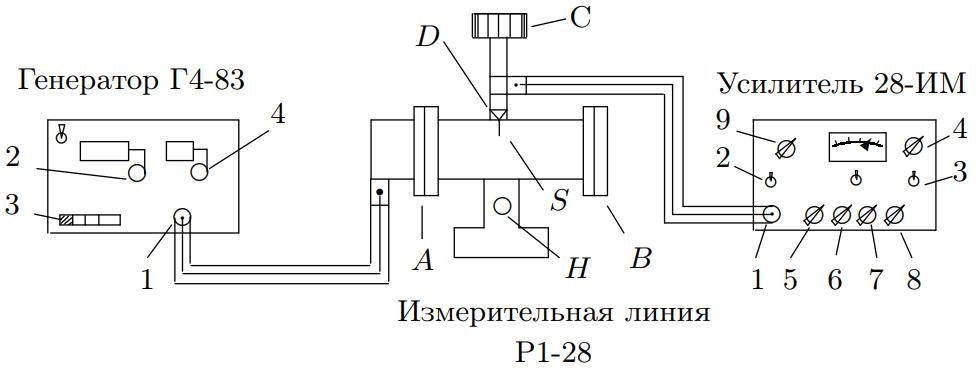
\includegraphics[width=13.5cm, height=5.3cm]{images/scheme1.jpg}
    \caption{Экспериментальная установка для изучения структуры волн СВЧ}
    \label{fig:scheme}
\end{figure}
С нагрузки детектора (c RC-цепочки) снимается огибающая высокочастотного сигнала и подаётся на усилитель низкой частоты. Величина сигнала регистрируется вольтметром, вмонтированным в усилитель. Ручка C — настройка измерительной линии — служит для согласования зонда (как антенны) со входом усилителя. Как правило, они согласованы, и в настройке нет необходимости. В волноводе с закрытым выходом образуется стоячая волна. Определив расстояние между узлами, можно рассчитать длину волны и фазовую скорость СВЧ-сигнала в волноводе. Устройство детекторной головки, установленной на измерительной линии, таково, что отклик вольтметра U на величину напряжённости электрического поля E в волноводе $U \sim E^n$, а показатель степени $n$ сам зависит от величины сигнала: при малых сигналах детектирование квадратичное ($n = 2$), при больших — линейное ($n = 1$). Если известно распределение поля $E(z)$ вдоль измерительной линии, то, изучив распределение $U(z)$, можно по графику $ln(U) = f[ln(E)]$ определить характер детектирования: в двойном логарифмическом масштабе любая степенная функция — прямая линия, по наклону которой можно определить $n$. Распределение E(z) нетрудно рассчитать для волновода с закороченным концом (металлической заглушкой), когда фаза отражённой волны $\varphi = \pi$, а $\rho = 1$.\\
Как следует из выражений напряжённости электрического поля, полученных выше, электрическое поле в этом случае имеет вид:

\begin{equation}
    E(z) = E_0 e^{-i k_z z} (1 - e^{2 i k_z z}) e^{i \omega t} = E_0 e^{i \omega t} (e^{-i k_z z} - e^{i k_z z}) = 2 E_0 e^{i \omega t} \sin (k_z z) \sim \sin (k_z z)
\end{equation}
где $z$ - смещение от узла. Меняя нагрузку на выходе измерительной линии (на рис. 2) и сравнивая максимальное и минимальное показания вольтметра, можно рассчитать коэффициент стоячей волны (к.с.в.) и коэффициент отражения $\rho$.






\section*{Ход работы}
В первую очередь подготавливаем все приборы к работе. \\

\textbf{Определение длины волны СВЧ-сигнала в волноводе.}\\
Восстанавливаем рабочую частоту $\nu = 9320$ МГц. Перемещая зонд, настраиваемся на пучность стоячей волны. Далее с помощью переключаталей 5 и 9 подобрали чувствительность вольтметра так, чтобы в максимуме стрелка отклонялась почти на всю шкалу. Используя весь возможный диапазон перемещения зонда вдоль измерительной линии, снимем зависимость показаний вольметра $U$ от положения зонда $z$:

\begin{table}[H]

    \centering
	\begin{tabular}{|c|c|c|c|}
		\hline
		\text{№} & $z,\ \text{мм}$ & $U,\ \text{дел}$ &  $U,\ \text{мкВ}$ \\
		\hline
		1.  & 10 & 27 & 2700 \\
		2.  & 0 & 32 & 3200 \\
		3.  & 4 & 1 & 100 \\
		4.  & 8 & 11  & 1100 \\
		5.  & 12 & 53  & 5300 \\
		6.  & 16 & 89  & 8900 \\
		7.  & 20 & 66 & 6600 \\
		8.  & 24 & 11 & 1100 \\
		9.  & 28 & 0 & 0 \\
        10. & 32 & 24 & 2400 \\
        11. & 36 & 73 & 7300 \\
        12. & 40 & 87 & 8700 \\
		\hline
	\end{tabular}
 \caption{Зависимость $U$ от положения зонда $z$,\ k = 100 мкВ/дел}
\end{table}\\

\newpage
Теперь построим график $U = f(z)$ и определим по нему длину волны $\lambda_{\text{в}}$ в волноводе.

\begin{figure}[H]
    \centering
    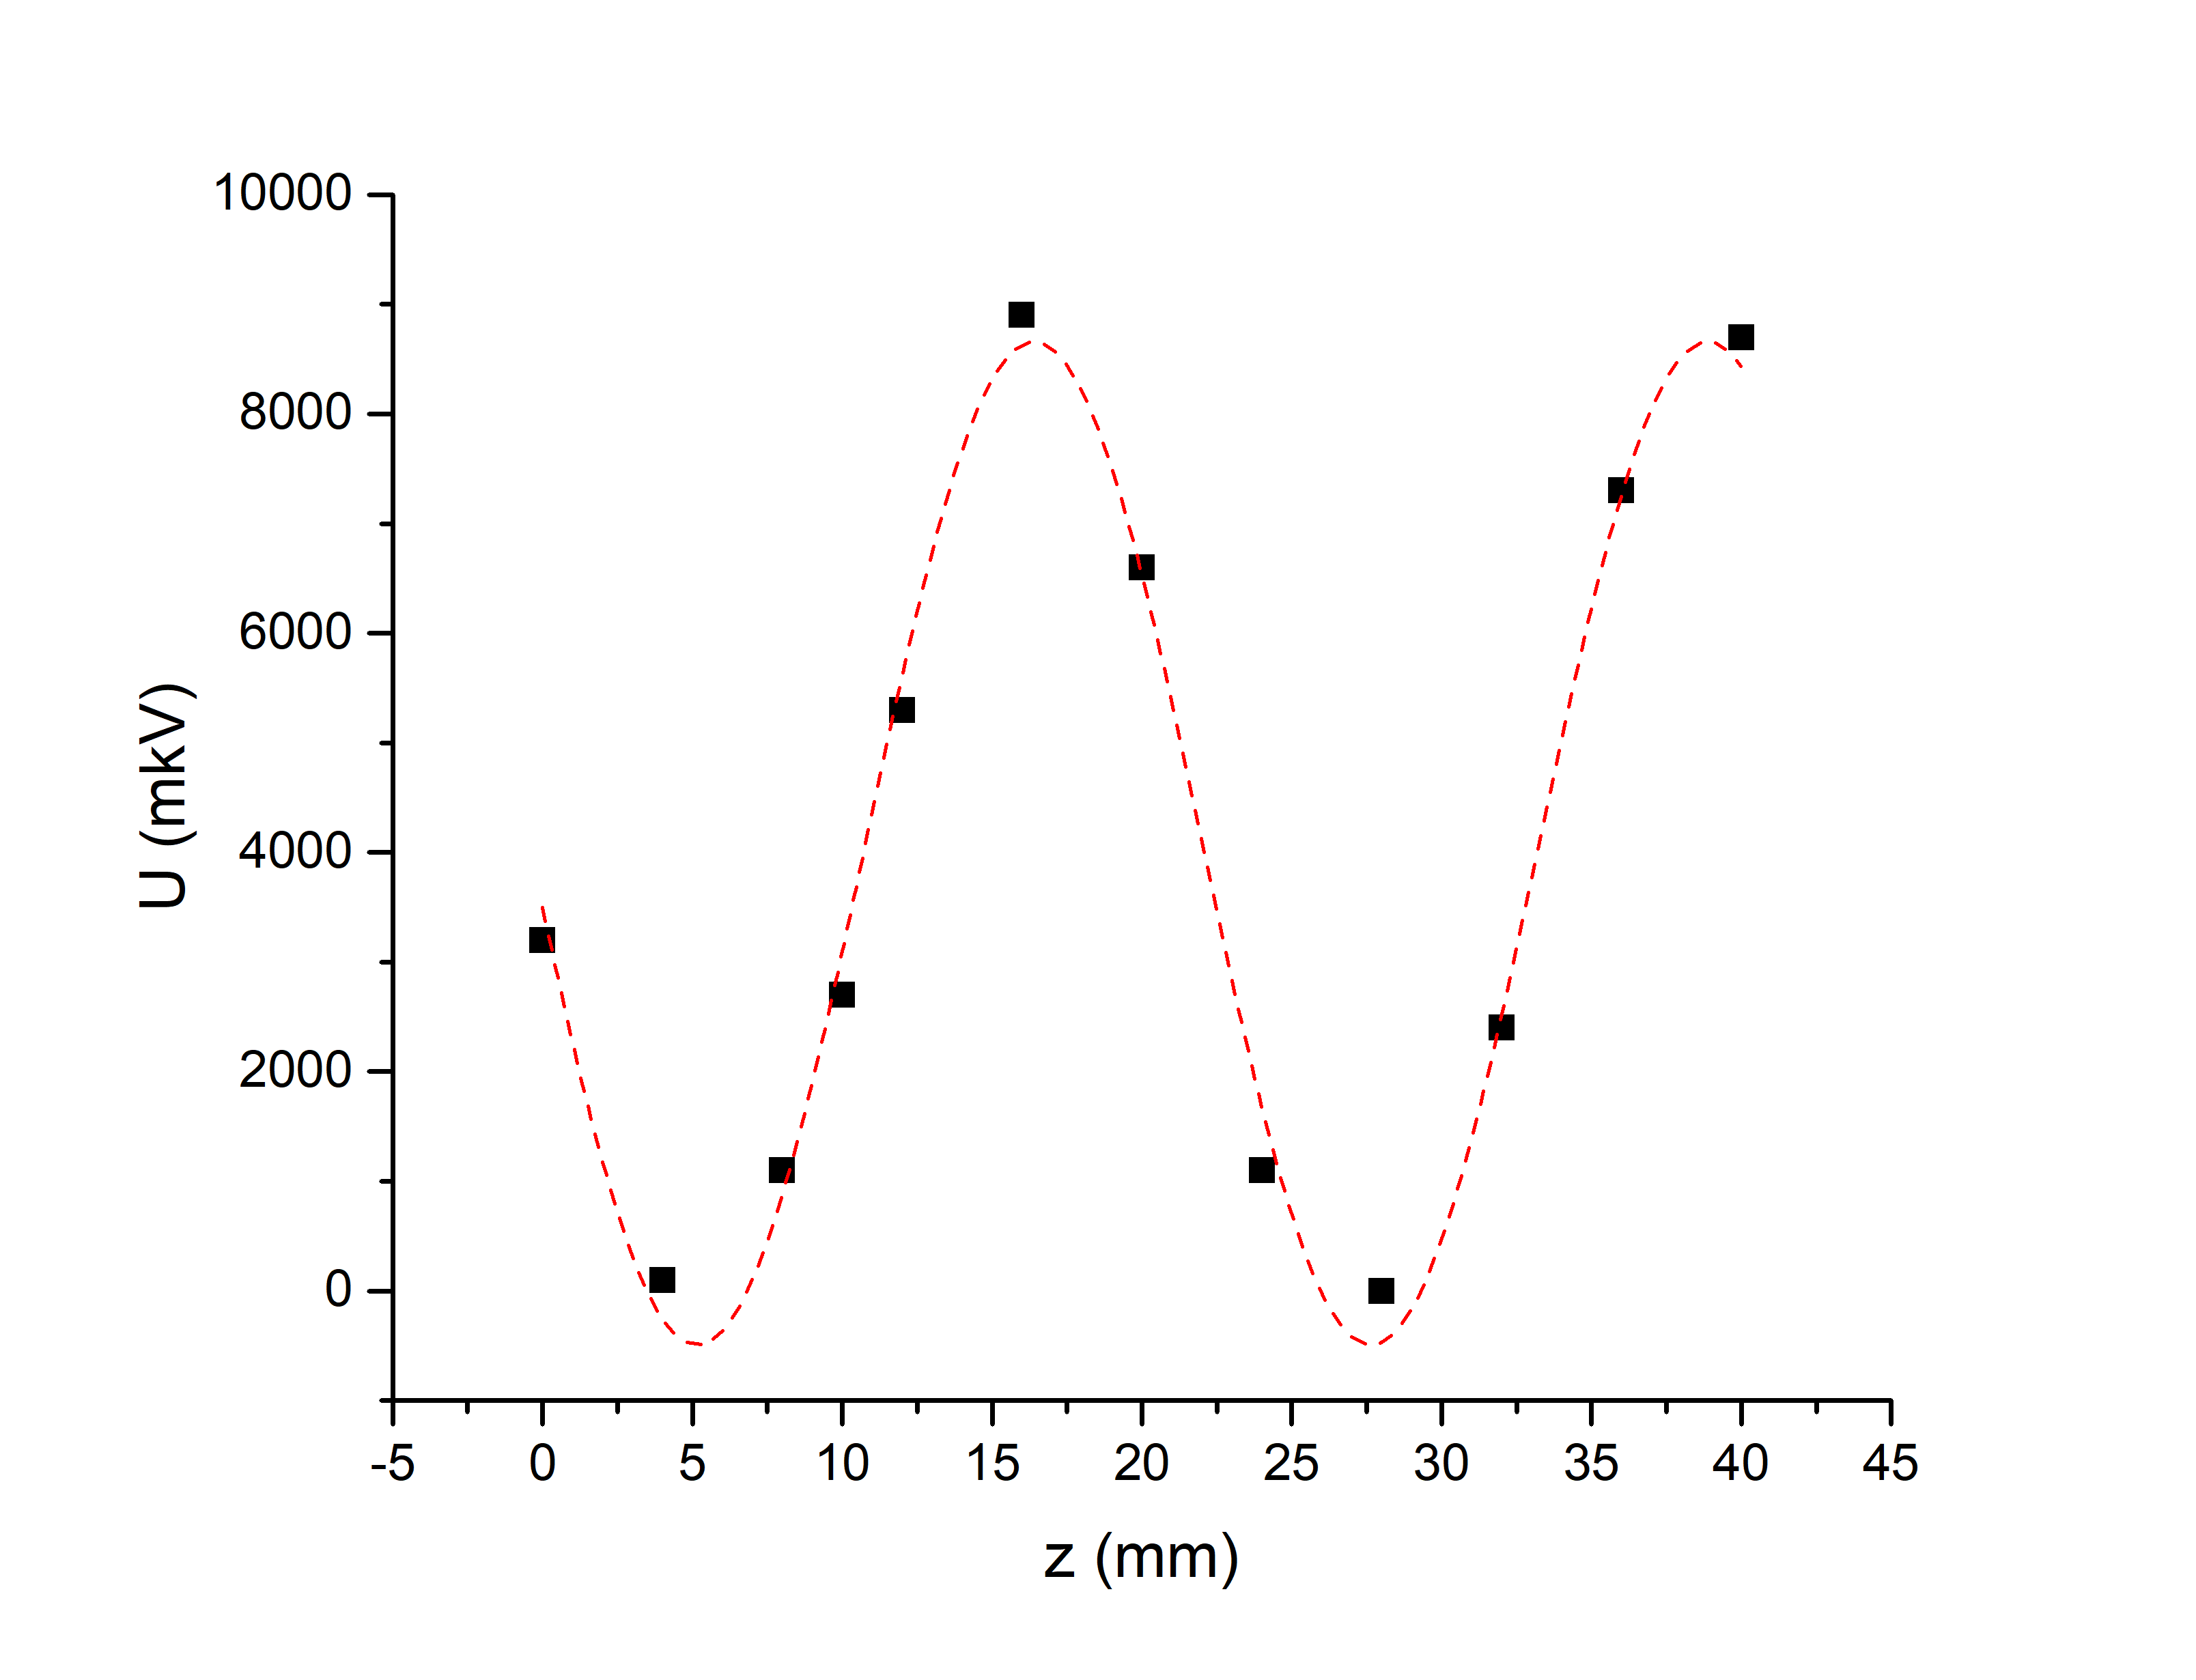
\includegraphics[width=13.5cm, height=8.8cm]{images/graph1.png}
\end{figure}


И получаем $\lambda_{\text{в}}$ = 45,2 мм. Теперь можем сравнить это с теоретическим расчётом: $\lambda_{\text{в}}$ = 45,1 мм. Результаты практически совпадают.

Сравним длину волны $\lambda_0$ в открытом пространстве с критической $\lambda_{\text{кр}}$:\\
$\lambda_0$ = 32,2 мм,\ $\lambda_{\text{кр}}$ = 46,0 мм.

Расчитаем фазовую скорость волн в волноводе и групповую скорость $u$, используя соотношение $uv_{\text{Ф}} = c^2$: $v_{\text{Ф}}$ = 1514925741 $\frac{\text{м}}{\text{с}} = 5,1c$,\ $u=0,198c$.\\

\textbf{Определение характера детектирования.}

Установим зонд в узел стоячей волны ($U = U_{min}$). Переключателями 5 и 9 подберём чувствительность вольметра так, чтобы отклонение стрелки было заметным. Снимем зависимость $U$ от координаты зонда внутри выбранного диапазона.

\begin{table}[H]
    \centering
	\begin{tabular}{|c|c|c|c|c|}
		\hline
		\text{№} & $z,\ \text{мм}$ & \Delta z,\ \text{мм} & $U,\ \text{дел}$ &  $U,\ \text{мкВ}$ \\
		\hline
		1.  & 25,5 & 2 & 91 & 546 \\
		2.  & 26,0 & 1,5 & 52 & 312 \\
		3.  & 26,5 & 1 & 24 & 144 \\
		4.  & 27,0 & 0,5& 9  & 54 \\
		5.  & 27,5 & 0& 2  & 12 \\
		6.  & 28,0 & 0,5& 6  & 36 \\
		7.  & 28,5 & 1& 20 & 120 \\
		8.  & 29,0 & 1,5& 41 & 246 \\
		9.  & 29,5 &2& 72 & 432 \\
		\hline
	\end{tabular}
 \caption{Зависимость $U$ от положения зонда $z$}
\end{table}\\

При этом $k = 6$ мкВ/дел, $z_{\text{узла}} = 27,5$ мм, $k_z = 0,00013945$ 1/м.\\

Построим график $ln(U) = f(ln(sin(k_zz)))$, где $z$ --- смещение от узла.

\begin{figure}[H]
    \centering
    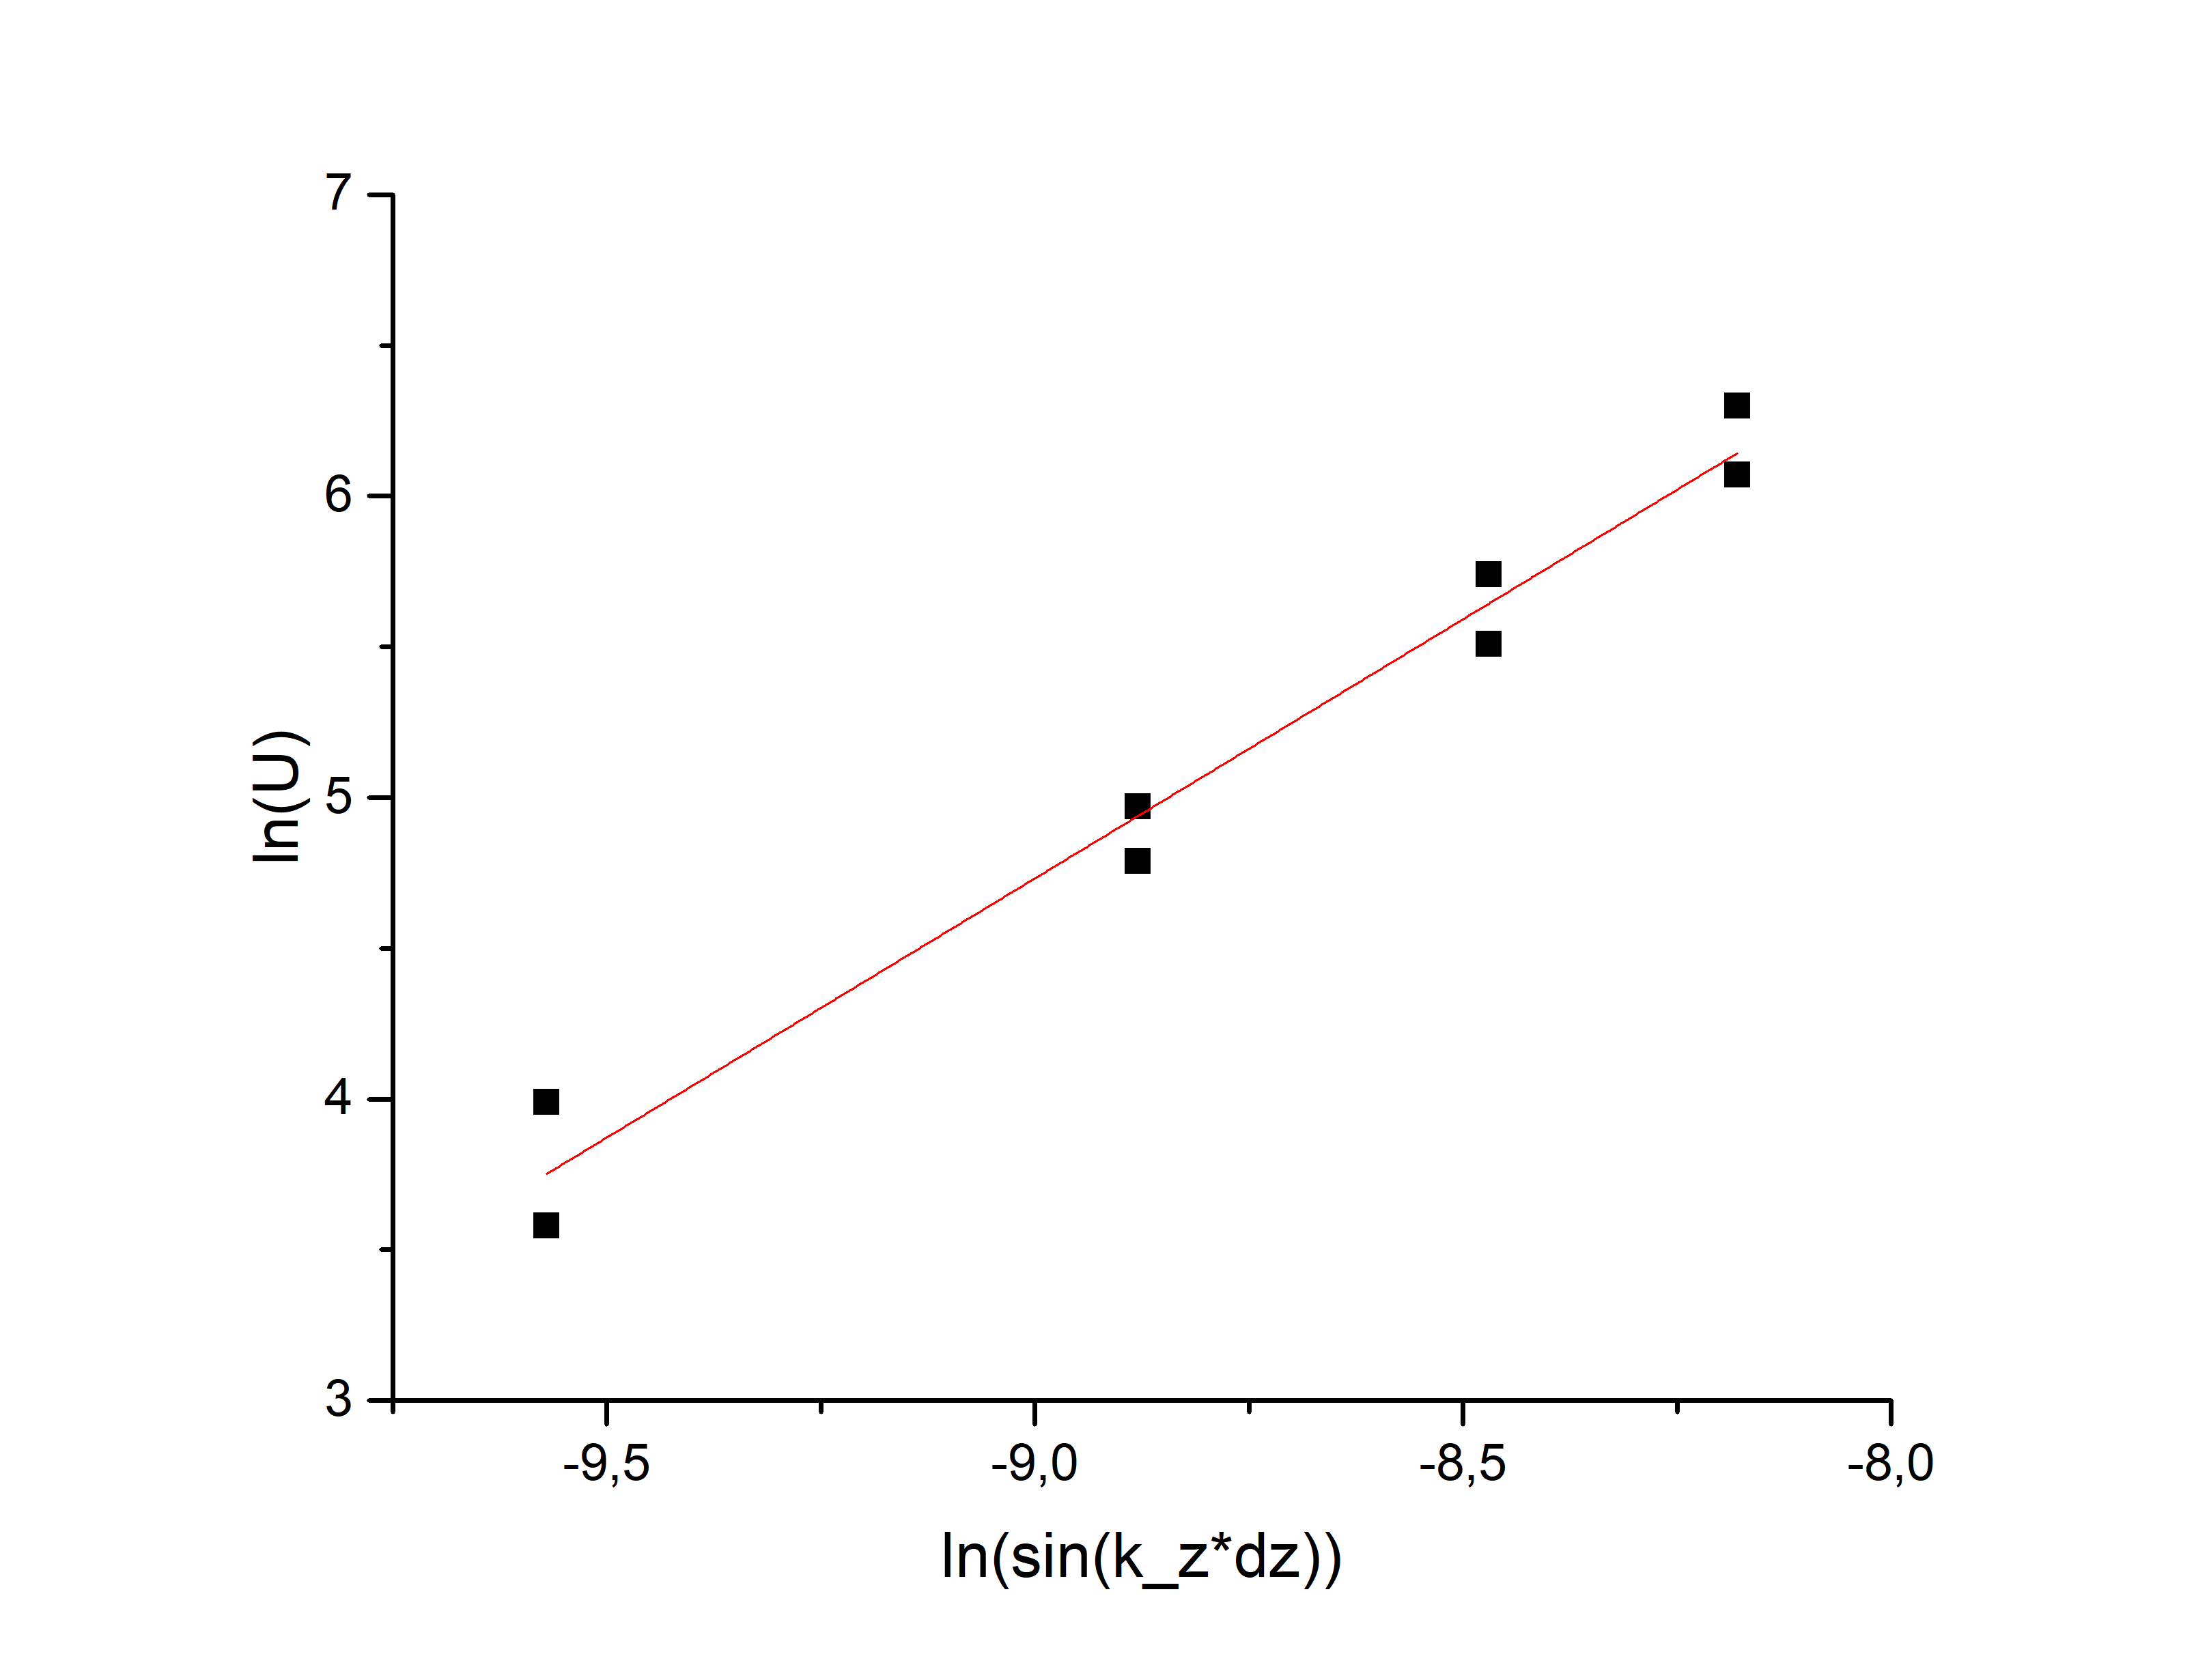
\includegraphics[width=13.5cm, height=8.8cm]{images/graph2.png}
\end{figure}

По наклону прямой теперь можем определить характер детектирования. Так как $k = 1,72$ ближе к двум, делаем вывод о том, что характер детектирования квадратичный.\\\\

\textbf{Определение коэффициентов отражения.}

Теперь снимем металлическую заглушку с фланца измерительной линии.  Перемещая зонд, измерим $U_{max}$ и $U_{min}$ напряжения в волне.

Потом наденем на выходной фланец измерительной линии отрезок волновода с поглощающей нагрузкой и снова измерим максимальное и минимальное напряжения.

Определим коэффициенты отражения $r$ для открытого, закрытого волновода и для волновода с поглощающей нагрузкой.

\begin{table}[H]
    \centering
	\begin{tabular}{|c|c|c|c|}
		\hline
		&U_{max},\ \text{мкВ} & U_{min},\ \text{мкВ} & r\\
		\hline
		  Отраж. заглушка  & 8800 & 24 & 0,99  \\
		Воздух  & 1860 & 540 & 0,55  \\
		Поглащ. нагрузка  & 1110 & 810 & 0,16 \\
		\hline
	\end{tabular}
 \caption{Определение коэффициентов отражения}
\end{table}\\

\newpage
\section*{Заключение}
В процессе выполнения лабораторной работы мы получили: \\
1) Длину волны в волноводе, близкую к теоретическому значению\\
2) Характер детектирования, близкий к квадратичному\\
3) Коэффициенты отражения, логически соответствующие ситуации, в которой они были получены.\\
Для улучшения результатов опыта стоило бы уделить больше внимания методу снятия напряжения вольтметром (данный нам вольтметр был старым и достаточно неточным, о чём говорили колебания его стрелки при отсутствии действий со стороны экспериментаторов). Но в целом, результаты эксперимента получились крайне логичными и соответствующими теории.


\section*{Литература}
\noindent
1. Сивухин Д. В. Общий курс физики. Учеб. пособие: Для вузов. Т. III. Электричество. - 6-е издание. М.: ФИЗМАТЛИТ, 2019 \\
2. Никулин М.Г., Попов П.В., Нозик А.А., и др. Лабораторный практикум по общей физике: учеб. пособие. В трёх томах. Т. II. Электричество и магнетизм. - 2-е издание. М.: МФТИ, 2019\\
3. Описание лабораторной работы с сайта МФТИ: clck.ru/37JNSv





\end{document}
